\subsubsection{08.12.14}

\begin{enumerate}
	\item The time of beginning and ending of the meeting:
	17:00 - 20:30
	\item Purposes of the meeting:
	\begin{enumerate}
	  \item To make the new bucket.
	  
	  \item To test the new bucket.
	  
    \end{enumerate}
	\item Work that has been done:
	\begin{enumerate}
	  \item We use as a material for bucket packaging of PET because we couldn't buy list of PET.
	  
	  \item Projection of bucket was cut out. Bucket was fastened by duct tape. We planned to strengthen it by superglue.
	  
	  \begin{figure}[H]
	  	\begin{minipage}[h]{0.31\linewidth}
	  		\center{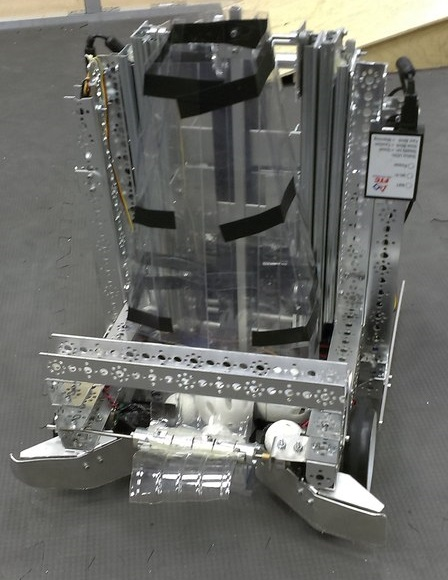
\includegraphics[scale=0.31]{days/08.12.14/images/01}}  
	  	\end{minipage}
	  	\hfill
	  	\begin{minipage}[h]{0.31\linewidth}
	  		\center{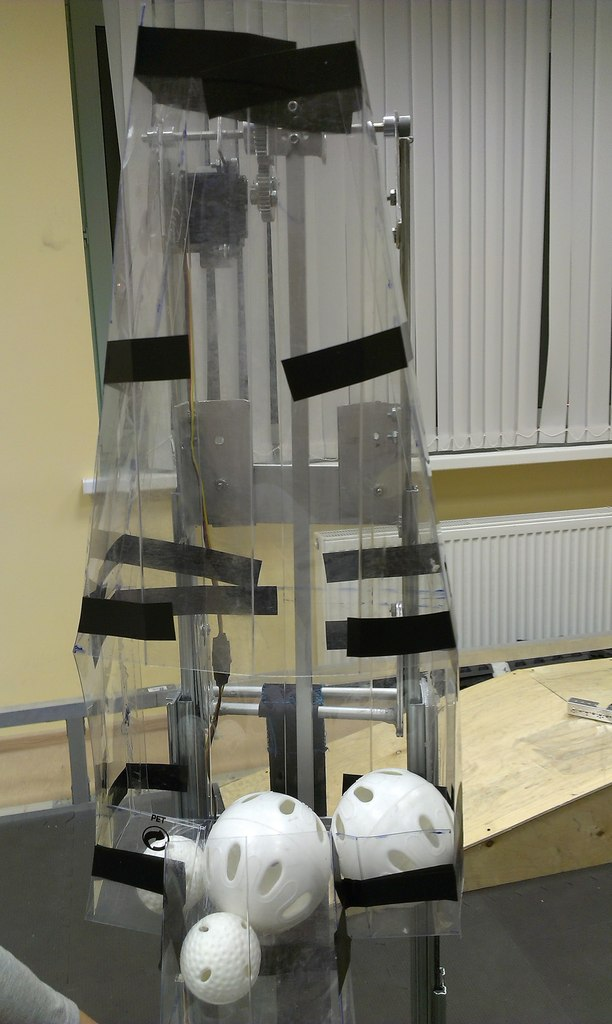
\includegraphics[scale=0.18]{days/08.12.14/images/02}} 
	  	\end{minipage}
	  	\hfill
	  	\begin{minipage}[h]{0.31\linewidth}
	  		\center{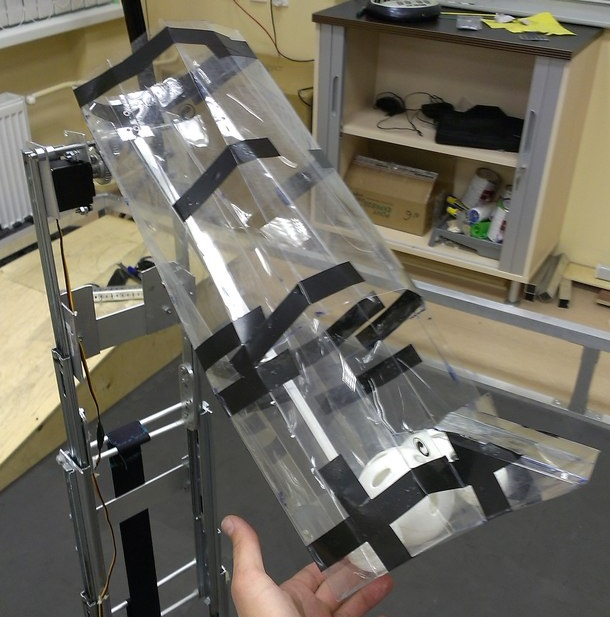
\includegraphics[scale=0.3]{days/08.12.14/images/03}}
	  	\end{minipage}
	  	\vfill
	    \caption{New bucket}
	  \end{figure}
      
      \item Bucket was tested for picking up balls. In most cases balls gets into the bucket. Some balls gets to the side and stuck on the robot. It was decided to make slopes which will prevent to balls get to side. Some balls doesn't leave the gripper and throws outside. It was decided to install limiters which prevent to balls move outside. Balls doesn't fall from the bucket after getting to it.
      
      \item It was turned out that small balls can get under the bottom of robot due to the increase of clearance. So the slopes were fixed lower.
      
      \item Bucket was bended due to the weight of balls. So it was fixed aluminium profile to back part of bucket. After that bucket stop to bend.
      
    \end{enumerate}
    
	\item Results:  
	\begin{enumerate}
	  \item Bucket was created and installed on the robot.
	  
	  \item Tests of bucket were succsessful.
	  
	  \item Slopes were fixed lower.
	  
    \end{enumerate}
    
	\item Tasks for the next meetings:
	\begin{enumerate}
	  \item To test MOB with the bucket.
	  
	  \item Install limiters that will prevent to balls move outside the bucket.
	  	  
    \end{enumerate}     
\end{enumerate}
